\section{Introduction}
\frame{\sectionpage}

\begin{frame}{Inspiration: The Puzzle of Spatial Attention and Dynamic Stimuli}
    \uncover<+->{How spatial attention impacts the neural processing of dynamic visual stimuli} \uncover<+->{is \textcolor{lightlavender}{\textbf{unclear}}}
    
    \uncover<2->{\hfill {\scriptsize See \cite{nobre2018anticipated} for a review}}
    
    \vspace{10pt}
    \only<3->{
    2 \textbf{\textcolor{lightlavender}{opposing}} functions in the perception of dynamic visual stimuli
        \begin{itemize}
            \item<3-> \textbf{\textcolor{lightlavender}{\underline{integration}:}} to form unitary percepts and identify \textcolor{lightlavender}{consistencies}
            \item<4-> \textbf{\textcolor{lightlavender}{\underline{segragation}:}} to parse separate objects and identify \textcolor{lightlavender}{changes}
        \end{itemize}
    }
    
\end{frame}

\begin{frame}{Inspiration: The Puzzle of Spatial Attention and Dynamic Stimuli}

    Surprisingly, spatial attention can \textbf{\textcolor{lightlavender}{flexibly}} benefit both:
    
    \begin{columns}[T]

        \begin{column}{0.45\textwidth}
            \uncover<2->{\begin{block}{\small \centering \textbf{Integration}}
            \uncover<3->{\footnotesize
            \begin{itemize}
                \item[-] \citet{hein2006visual}
                \item[-] \citet{sharp2018endogenous}
            \end{itemize}
            }
            \end{block}}
        \end{column}
        
        \begin{column}{0.45\textwidth}
            \uncover<2->{\begin{block}{\small \centering \textbf{Separation}}
            \uncover<3->{\footnotesize
            \begin{itemize}
                \item[-] \citet{akyurek2007adaptive}
                \item[-] \citet{hochmitz2021effects}
            \end{itemize}
            }
            \end{block}}
        \end{column}
        
        \end{columns}
    
        \vspace{15pt}
        \uncover<4->{How can spatial attention achieve this?}
    
\end{frame}


\begin{frame}{{Hypothesis:} The Measure of Corruption}

    \uncover<+->{\textcolor{lightlavender}{\textbf{Hypothesis:}}} The impact of \textcolor<13>{lightlavender}{\textbf{spatial attention on temporal processing}} is instantiated in part through effects on \textcolor<9-12>{lightlavender}{$\alpha$ \textbf{frequency}} in \textcolor<2-7>{lightlavender}{\textbf{retinotopic visual cortex}}.
    
    \only<2-7>{
        \begin{columns}

            \begin{column}{0.45\textwidth}
                \begin{figure}\label{fig1}
                \centering
                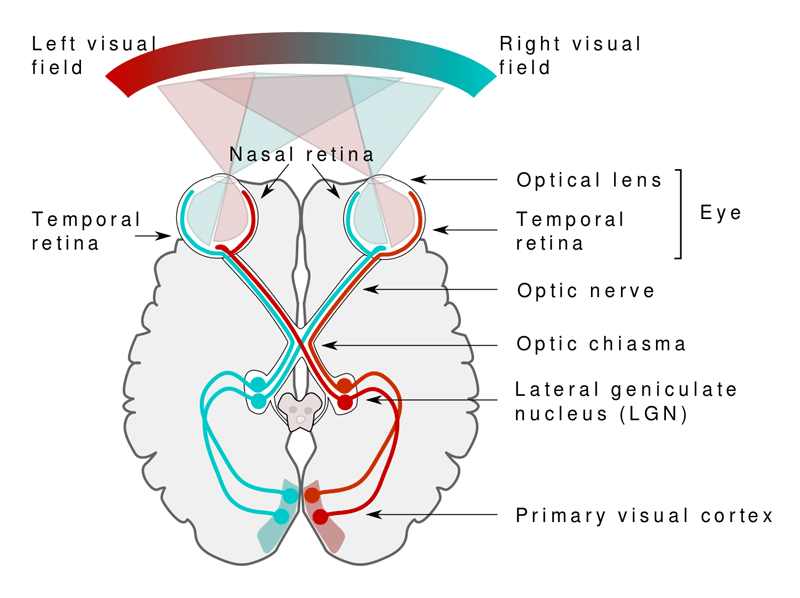
\includegraphics[height = 0.5 \textheight]{images/fig1.png}
                \caption{Retinotopic structure}
                \end{figure}
            \end{column}
            
            \begin{column}{0.5\textwidth}
            
            \begin{itemize}
                  \item<3-> \textcolor{lightlavender}{\textbf{striate}} and \textcolor{lightlavender}{\textbf{extrastriate}} visual areas: spatially organized, corresponding to specific areas of the retina
                  \item<4-> representing \textcolor{lightlavender}{\textbf{static}} stimuli: Yes!
                  \item<5-> representing \textcolor{lightlavender}{\textbf{temporal}} stimuli\only<5>{?}\only<6->{: \textcolor<7>{lightlavender}{\textit{shrinking/stretching the temporal scope of visual input summarizing}}}
              \end{itemize}
            
            \end{column}
            \end{columns}
    }

    \only<8-12>{
        \hfill \textcolor{lightlavender}{\textit{shrinking/stretching}} \textit{the temporal scope of visual input summarizing}
        
        \vspace*{15pt}
        \begin{itemize}
            \item<10-> $\alpha$ rate reflects \textcolor{lightlavender}{\textbf{temporal}} expectation 
            
            {\scriptsize See \citet{samaha2015speed,buergers2022role}}
            \item<11-> manipulation of average $\alpha$ rate has an impact on stretching/shrinking of the perceptual window
            
            {\scriptsize See \citet{cecere2015individual,minami2017illusory,ronconi2018alpha,mioni2020modulation}}
            \item<12-> average $\alpha$ rate (immediately before stimuli) becomes \textcolor{lightlavender}{\textbf{faster}} for segregation;  \textcolor{lightlavender}{\textbf{slower}} for integration
            
            {\scriptsize See \citet{wutz2018frequency}}
        \end{itemize}
    }

    \only<13->{
        \begin{itemize}
            \item<13-> \underline{\textbf{spatial}}: cue location $\Rightarrow$ \textit{corresponding} location in retinotopic visual cortex
            \item<14-> \underline{\textbf{temporal}}: segragation/integration $\Rightarrow$ $\alpha-$frequency faster or slower
        \end{itemize}
    }
        
    \end{frame}

    \begin{frame}{{Prediction:} The Measure of Corruption}

        \only<+->{
            \begin{columns}
    
                \begin{column}{0.45\textwidth}
                    \begin{figure}
                    \centering
                    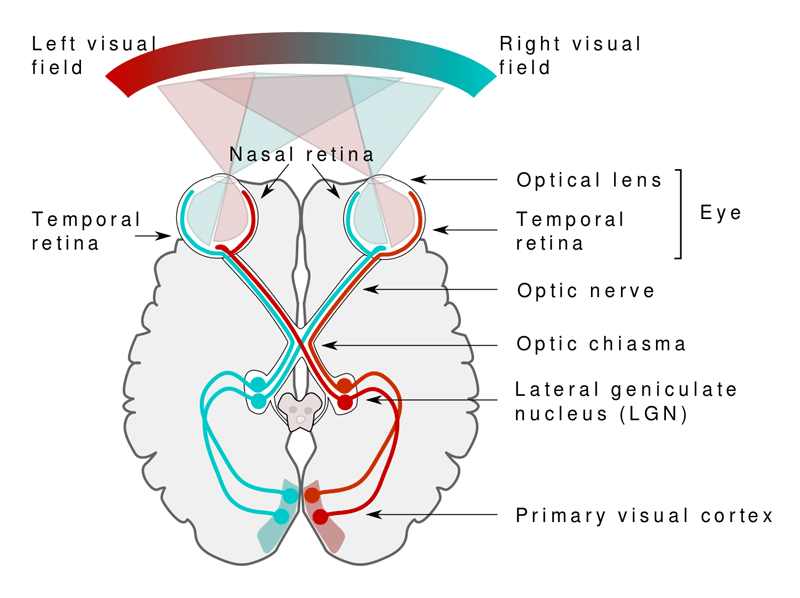
\includegraphics[height = 0.55 \textheight]{images/fig1.png}
                    \caption{Retinotopic structure}
                    \end{figure}
                \end{column}
                
                \begin{column}{0.5\textwidth}
                
                    \begin{table}[h!]
                        \footnotesize
                        \begin{center}
                          \label{tab:prediction}
                          \begin{tabular}{lcc}
                            
                            & \textcolor{lightlavender}{contralateral} & \textcolor{lightlavender}{ipsilateral}  \\
                            \hline
                            \textcolor{lightlavender}{segragation} & faster & \textit{slower} \\
                            \textcolor{lightlavender}{Integration} & slower & \textit{faster}
                          \end{tabular}
                        \end{center}
                      \end{table}

                    Use \textcolor{lightlavender}{magnetoencephalogram (MEG)} recording for analysis
                
                \end{column}
                \end{columns}
        }
            
        \end{frame}